\section{Results}
Using some \textit{api} from Castalia Simulator some results like the total number of control packets exchanged, the total number of measurements packets, how many times a packets was retransmited among many others results can be obtained easily.

\subsection{Use case and simulation parameters}

Monitoring and Independent living for elder care is one of the use context of 11073 standard. The sensors and devices used for this use case is described in \cite{b3} is blood pressure, thermometer, glucose meter, pulse oximeter and basic ECG. In this work we used a hypothetical elderly patient who has cardiac problems, diabetes and hypertension and  after a major surgery needs to be monitored in his home.

The Fig.~\ref{fig:wbantopology} shows the topology setup used in our simulation. The hub node is placed at the right hip, one sensor node at the right and left wrist, one sensor node at the right and left ankle and one sensor on chest. The deployment of nodes is not the ideal, we just use this set to test our feature. The positions of nodes was maintained as they are in Castalia because real experimental measurements of path loss was made for every pair of nodes in \cite{b4}.

\begin{figure}[htbp]
\centerline{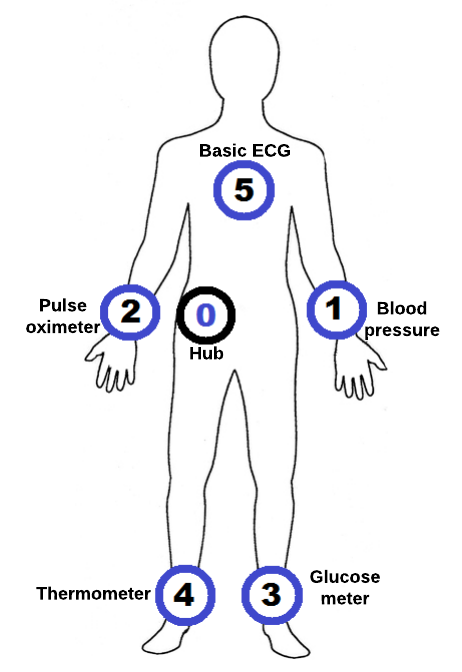
\includegraphics[scale=0.31]{figures/corpoSensoresNomes.png}}
\caption{The simulated network topology.}
\label{fig:wbantopology}
\end{figure}

In this paper we will simulate two scenario. The first scenario the agents will send measurement with no confirmation and the second with confirmation from the manager. The MAC layer used is the IEEE 802.15.6 with path loss map and temporal model for wireless channel supplied by Castalia and 1024 Kbps of physical data rate. The radio used meets with the IEEE 802.15.6 radio proposal \cite{5} and -15dBm as transmission power.

The node 0 uses the \textit{Manager} application and is the hub. The blood pressure and the pulse oximeter transmit one measurement per second. The thermometer convey one read every 2 seconds. The glucose meter  transmit one measurement every twenty five seconds. In this work we assume the basic ECG is a device that receives the signals of all electrodes deployed in the body and transmit these signals to the Manager.  